
% Default to the notebook output style

    


% Inherit from the specified cell style.




    
\documentclass[11pt]{article}

    
    
    \usepackage[T1]{fontenc}
    % Nicer default font (+ math font) than Computer Modern for most use cases
    \usepackage{mathpazo}

    % Basic figure setup, for now with no caption control since it's done
    % automatically by Pandoc (which extracts ![](path) syntax from Markdown).
    \usepackage{graphicx}
    % We will generate all images so they have a width \maxwidth. This means
    % that they will get their normal width if they fit onto the page, but
    % are scaled down if they would overflow the margins.
    \makeatletter
    \def\maxwidth{\ifdim\Gin@nat@width>\linewidth\linewidth
    \else\Gin@nat@width\fi}
    \makeatother
    \let\Oldincludegraphics\includegraphics
    % Set max figure width to be 80% of text width, for now hardcoded.
    \renewcommand{\includegraphics}[1]{\Oldincludegraphics[width=.8\maxwidth]{#1}}
    % Ensure that by default, figures have no caption (until we provide a
    % proper Figure object with a Caption API and a way to capture that
    % in the conversion process - todo).
    \usepackage{caption}
    \DeclareCaptionLabelFormat{nolabel}{}
    \captionsetup{labelformat=nolabel}

    \usepackage{adjustbox} % Used to constrain images to a maximum size 
    \usepackage{xcolor} % Allow colors to be defined
    \usepackage{enumerate} % Needed for markdown enumerations to work
    \usepackage{geometry} % Used to adjust the document margins
    \usepackage{amsmath} % Equations
    \usepackage{amssymb} % Equations
    \usepackage{textcomp} % defines textquotesingle
    % Hack from http://tex.stackexchange.com/a/47451/13684:
    \AtBeginDocument{%
        \def\PYZsq{\textquotesingle}% Upright quotes in Pygmentized code
    }
    \usepackage{upquote} % Upright quotes for verbatim code
    \usepackage{eurosym} % defines \euro
    \usepackage[mathletters]{ucs} % Extended unicode (utf-8) support
    \usepackage[utf8x]{inputenc} % Allow utf-8 characters in the tex document
    \usepackage{fancyvrb} % verbatim replacement that allows latex
    \usepackage{grffile} % extends the file name processing of package graphics 
                         % to support a larger range 
    % The hyperref package gives us a pdf with properly built
    % internal navigation ('pdf bookmarks' for the table of contents,
    % internal cross-reference links, web links for URLs, etc.)
    \usepackage{hyperref}
    \usepackage{longtable} % longtable support required by pandoc >1.10
    \usepackage{booktabs}  % table support for pandoc > 1.12.2
    \usepackage[inline]{enumitem} % IRkernel/repr support (it uses the enumerate* environment)
    \usepackage[normalem]{ulem} % ulem is needed to support strikethroughs (\sout)
                                % normalem makes italics be italics, not underlines
    

    
    
    % Colors for the hyperref package
    \definecolor{urlcolor}{rgb}{0,.145,.698}
    \definecolor{linkcolor}{rgb}{.71,0.21,0.01}
    \definecolor{citecolor}{rgb}{.12,.54,.11}

    % ANSI colors
    \definecolor{ansi-black}{HTML}{3E424D}
    \definecolor{ansi-black-intense}{HTML}{282C36}
    \definecolor{ansi-red}{HTML}{E75C58}
    \definecolor{ansi-red-intense}{HTML}{B22B31}
    \definecolor{ansi-green}{HTML}{00A250}
    \definecolor{ansi-green-intense}{HTML}{007427}
    \definecolor{ansi-yellow}{HTML}{DDB62B}
    \definecolor{ansi-yellow-intense}{HTML}{B27D12}
    \definecolor{ansi-blue}{HTML}{208FFB}
    \definecolor{ansi-blue-intense}{HTML}{0065CA}
    \definecolor{ansi-magenta}{HTML}{D160C4}
    \definecolor{ansi-magenta-intense}{HTML}{A03196}
    \definecolor{ansi-cyan}{HTML}{60C6C8}
    \definecolor{ansi-cyan-intense}{HTML}{258F8F}
    \definecolor{ansi-white}{HTML}{C5C1B4}
    \definecolor{ansi-white-intense}{HTML}{A1A6B2}

    % commands and environments needed by pandoc snippets
    % extracted from the output of `pandoc -s`
    \providecommand{\tightlist}{%
      \setlength{\itemsep}{0pt}\setlength{\parskip}{0pt}}
    \DefineVerbatimEnvironment{Highlighting}{Verbatim}{commandchars=\\\{\}}
    % Add ',fontsize=\small' for more characters per line
    \newenvironment{Shaded}{}{}
    \newcommand{\KeywordTok}[1]{\textcolor[rgb]{0.00,0.44,0.13}{\textbf{{#1}}}}
    \newcommand{\DataTypeTok}[1]{\textcolor[rgb]{0.56,0.13,0.00}{{#1}}}
    \newcommand{\DecValTok}[1]{\textcolor[rgb]{0.25,0.63,0.44}{{#1}}}
    \newcommand{\BaseNTok}[1]{\textcolor[rgb]{0.25,0.63,0.44}{{#1}}}
    \newcommand{\FloatTok}[1]{\textcolor[rgb]{0.25,0.63,0.44}{{#1}}}
    \newcommand{\CharTok}[1]{\textcolor[rgb]{0.25,0.44,0.63}{{#1}}}
    \newcommand{\StringTok}[1]{\textcolor[rgb]{0.25,0.44,0.63}{{#1}}}
    \newcommand{\CommentTok}[1]{\textcolor[rgb]{0.38,0.63,0.69}{\textit{{#1}}}}
    \newcommand{\OtherTok}[1]{\textcolor[rgb]{0.00,0.44,0.13}{{#1}}}
    \newcommand{\AlertTok}[1]{\textcolor[rgb]{1.00,0.00,0.00}{\textbf{{#1}}}}
    \newcommand{\FunctionTok}[1]{\textcolor[rgb]{0.02,0.16,0.49}{{#1}}}
    \newcommand{\RegionMarkerTok}[1]{{#1}}
    \newcommand{\ErrorTok}[1]{\textcolor[rgb]{1.00,0.00,0.00}{\textbf{{#1}}}}
    \newcommand{\NormalTok}[1]{{#1}}
    
    % Additional commands for more recent versions of Pandoc
    \newcommand{\ConstantTok}[1]{\textcolor[rgb]{0.53,0.00,0.00}{{#1}}}
    \newcommand{\SpecialCharTok}[1]{\textcolor[rgb]{0.25,0.44,0.63}{{#1}}}
    \newcommand{\VerbatimStringTok}[1]{\textcolor[rgb]{0.25,0.44,0.63}{{#1}}}
    \newcommand{\SpecialStringTok}[1]{\textcolor[rgb]{0.73,0.40,0.53}{{#1}}}
    \newcommand{\ImportTok}[1]{{#1}}
    \newcommand{\DocumentationTok}[1]{\textcolor[rgb]{0.73,0.13,0.13}{\textit{{#1}}}}
    \newcommand{\AnnotationTok}[1]{\textcolor[rgb]{0.38,0.63,0.69}{\textbf{\textit{{#1}}}}}
    \newcommand{\CommentVarTok}[1]{\textcolor[rgb]{0.38,0.63,0.69}{\textbf{\textit{{#1}}}}}
    \newcommand{\VariableTok}[1]{\textcolor[rgb]{0.10,0.09,0.49}{{#1}}}
    \newcommand{\ControlFlowTok}[1]{\textcolor[rgb]{0.00,0.44,0.13}{\textbf{{#1}}}}
    \newcommand{\OperatorTok}[1]{\textcolor[rgb]{0.40,0.40,0.40}{{#1}}}
    \newcommand{\BuiltInTok}[1]{{#1}}
    \newcommand{\ExtensionTok}[1]{{#1}}
    \newcommand{\PreprocessorTok}[1]{\textcolor[rgb]{0.74,0.48,0.00}{{#1}}}
    \newcommand{\AttributeTok}[1]{\textcolor[rgb]{0.49,0.56,0.16}{{#1}}}
    \newcommand{\InformationTok}[1]{\textcolor[rgb]{0.38,0.63,0.69}{\textbf{\textit{{#1}}}}}
    \newcommand{\WarningTok}[1]{\textcolor[rgb]{0.38,0.63,0.69}{\textbf{\textit{{#1}}}}}
    
    
    % Define a nice break command that doesn't care if a line doesn't already
    % exist.
    \def\br{\hspace*{\fill} \\* }
    % Math Jax compatability definitions
    \def\gt{>}
    \def\lt{<}
    % Document parameters
    \title{Face\_Recognition\_Challenge\_Parth\_S\_Patel}
    
    
    

    % Pygments definitions
    
\makeatletter
\def\PY@reset{\let\PY@it=\relax \let\PY@bf=\relax%
    \let\PY@ul=\relax \let\PY@tc=\relax%
    \let\PY@bc=\relax \let\PY@ff=\relax}
\def\PY@tok#1{\csname PY@tok@#1\endcsname}
\def\PY@toks#1+{\ifx\relax#1\empty\else%
    \PY@tok{#1}\expandafter\PY@toks\fi}
\def\PY@do#1{\PY@bc{\PY@tc{\PY@ul{%
    \PY@it{\PY@bf{\PY@ff{#1}}}}}}}
\def\PY#1#2{\PY@reset\PY@toks#1+\relax+\PY@do{#2}}

\expandafter\def\csname PY@tok@nc\endcsname{\let\PY@bf=\textbf\def\PY@tc##1{\textcolor[rgb]{0.00,0.00,1.00}{##1}}}
\expandafter\def\csname PY@tok@si\endcsname{\let\PY@bf=\textbf\def\PY@tc##1{\textcolor[rgb]{0.73,0.40,0.53}{##1}}}
\expandafter\def\csname PY@tok@gt\endcsname{\def\PY@tc##1{\textcolor[rgb]{0.00,0.27,0.87}{##1}}}
\expandafter\def\csname PY@tok@kr\endcsname{\let\PY@bf=\textbf\def\PY@tc##1{\textcolor[rgb]{0.00,0.50,0.00}{##1}}}
\expandafter\def\csname PY@tok@ge\endcsname{\let\PY@it=\textit}
\expandafter\def\csname PY@tok@dl\endcsname{\def\PY@tc##1{\textcolor[rgb]{0.73,0.13,0.13}{##1}}}
\expandafter\def\csname PY@tok@cpf\endcsname{\let\PY@it=\textit\def\PY@tc##1{\textcolor[rgb]{0.25,0.50,0.50}{##1}}}
\expandafter\def\csname PY@tok@gu\endcsname{\let\PY@bf=\textbf\def\PY@tc##1{\textcolor[rgb]{0.50,0.00,0.50}{##1}}}
\expandafter\def\csname PY@tok@nb\endcsname{\def\PY@tc##1{\textcolor[rgb]{0.00,0.50,0.00}{##1}}}
\expandafter\def\csname PY@tok@fm\endcsname{\def\PY@tc##1{\textcolor[rgb]{0.00,0.00,1.00}{##1}}}
\expandafter\def\csname PY@tok@mb\endcsname{\def\PY@tc##1{\textcolor[rgb]{0.40,0.40,0.40}{##1}}}
\expandafter\def\csname PY@tok@sd\endcsname{\let\PY@it=\textit\def\PY@tc##1{\textcolor[rgb]{0.73,0.13,0.13}{##1}}}
\expandafter\def\csname PY@tok@sx\endcsname{\def\PY@tc##1{\textcolor[rgb]{0.00,0.50,0.00}{##1}}}
\expandafter\def\csname PY@tok@kn\endcsname{\let\PY@bf=\textbf\def\PY@tc##1{\textcolor[rgb]{0.00,0.50,0.00}{##1}}}
\expandafter\def\csname PY@tok@vc\endcsname{\def\PY@tc##1{\textcolor[rgb]{0.10,0.09,0.49}{##1}}}
\expandafter\def\csname PY@tok@ne\endcsname{\let\PY@bf=\textbf\def\PY@tc##1{\textcolor[rgb]{0.82,0.25,0.23}{##1}}}
\expandafter\def\csname PY@tok@sa\endcsname{\def\PY@tc##1{\textcolor[rgb]{0.73,0.13,0.13}{##1}}}
\expandafter\def\csname PY@tok@cm\endcsname{\let\PY@it=\textit\def\PY@tc##1{\textcolor[rgb]{0.25,0.50,0.50}{##1}}}
\expandafter\def\csname PY@tok@kt\endcsname{\def\PY@tc##1{\textcolor[rgb]{0.69,0.00,0.25}{##1}}}
\expandafter\def\csname PY@tok@ow\endcsname{\let\PY@bf=\textbf\def\PY@tc##1{\textcolor[rgb]{0.67,0.13,1.00}{##1}}}
\expandafter\def\csname PY@tok@mf\endcsname{\def\PY@tc##1{\textcolor[rgb]{0.40,0.40,0.40}{##1}}}
\expandafter\def\csname PY@tok@kc\endcsname{\let\PY@bf=\textbf\def\PY@tc##1{\textcolor[rgb]{0.00,0.50,0.00}{##1}}}
\expandafter\def\csname PY@tok@gi\endcsname{\def\PY@tc##1{\textcolor[rgb]{0.00,0.63,0.00}{##1}}}
\expandafter\def\csname PY@tok@s2\endcsname{\def\PY@tc##1{\textcolor[rgb]{0.73,0.13,0.13}{##1}}}
\expandafter\def\csname PY@tok@sh\endcsname{\def\PY@tc##1{\textcolor[rgb]{0.73,0.13,0.13}{##1}}}
\expandafter\def\csname PY@tok@go\endcsname{\def\PY@tc##1{\textcolor[rgb]{0.53,0.53,0.53}{##1}}}
\expandafter\def\csname PY@tok@na\endcsname{\def\PY@tc##1{\textcolor[rgb]{0.49,0.56,0.16}{##1}}}
\expandafter\def\csname PY@tok@k\endcsname{\let\PY@bf=\textbf\def\PY@tc##1{\textcolor[rgb]{0.00,0.50,0.00}{##1}}}
\expandafter\def\csname PY@tok@bp\endcsname{\def\PY@tc##1{\textcolor[rgb]{0.00,0.50,0.00}{##1}}}
\expandafter\def\csname PY@tok@nt\endcsname{\let\PY@bf=\textbf\def\PY@tc##1{\textcolor[rgb]{0.00,0.50,0.00}{##1}}}
\expandafter\def\csname PY@tok@s1\endcsname{\def\PY@tc##1{\textcolor[rgb]{0.73,0.13,0.13}{##1}}}
\expandafter\def\csname PY@tok@sr\endcsname{\def\PY@tc##1{\textcolor[rgb]{0.73,0.40,0.53}{##1}}}
\expandafter\def\csname PY@tok@gd\endcsname{\def\PY@tc##1{\textcolor[rgb]{0.63,0.00,0.00}{##1}}}
\expandafter\def\csname PY@tok@vg\endcsname{\def\PY@tc##1{\textcolor[rgb]{0.10,0.09,0.49}{##1}}}
\expandafter\def\csname PY@tok@sb\endcsname{\def\PY@tc##1{\textcolor[rgb]{0.73,0.13,0.13}{##1}}}
\expandafter\def\csname PY@tok@c\endcsname{\let\PY@it=\textit\def\PY@tc##1{\textcolor[rgb]{0.25,0.50,0.50}{##1}}}
\expandafter\def\csname PY@tok@mi\endcsname{\def\PY@tc##1{\textcolor[rgb]{0.40,0.40,0.40}{##1}}}
\expandafter\def\csname PY@tok@gr\endcsname{\def\PY@tc##1{\textcolor[rgb]{1.00,0.00,0.00}{##1}}}
\expandafter\def\csname PY@tok@nf\endcsname{\def\PY@tc##1{\textcolor[rgb]{0.00,0.00,1.00}{##1}}}
\expandafter\def\csname PY@tok@c1\endcsname{\let\PY@it=\textit\def\PY@tc##1{\textcolor[rgb]{0.25,0.50,0.50}{##1}}}
\expandafter\def\csname PY@tok@kp\endcsname{\def\PY@tc##1{\textcolor[rgb]{0.00,0.50,0.00}{##1}}}
\expandafter\def\csname PY@tok@gs\endcsname{\let\PY@bf=\textbf}
\expandafter\def\csname PY@tok@ch\endcsname{\let\PY@it=\textit\def\PY@tc##1{\textcolor[rgb]{0.25,0.50,0.50}{##1}}}
\expandafter\def\csname PY@tok@no\endcsname{\def\PY@tc##1{\textcolor[rgb]{0.53,0.00,0.00}{##1}}}
\expandafter\def\csname PY@tok@gp\endcsname{\let\PY@bf=\textbf\def\PY@tc##1{\textcolor[rgb]{0.00,0.00,0.50}{##1}}}
\expandafter\def\csname PY@tok@cs\endcsname{\let\PY@it=\textit\def\PY@tc##1{\textcolor[rgb]{0.25,0.50,0.50}{##1}}}
\expandafter\def\csname PY@tok@nv\endcsname{\def\PY@tc##1{\textcolor[rgb]{0.10,0.09,0.49}{##1}}}
\expandafter\def\csname PY@tok@vi\endcsname{\def\PY@tc##1{\textcolor[rgb]{0.10,0.09,0.49}{##1}}}
\expandafter\def\csname PY@tok@se\endcsname{\let\PY@bf=\textbf\def\PY@tc##1{\textcolor[rgb]{0.73,0.40,0.13}{##1}}}
\expandafter\def\csname PY@tok@sc\endcsname{\def\PY@tc##1{\textcolor[rgb]{0.73,0.13,0.13}{##1}}}
\expandafter\def\csname PY@tok@w\endcsname{\def\PY@tc##1{\textcolor[rgb]{0.73,0.73,0.73}{##1}}}
\expandafter\def\csname PY@tok@nn\endcsname{\let\PY@bf=\textbf\def\PY@tc##1{\textcolor[rgb]{0.00,0.00,1.00}{##1}}}
\expandafter\def\csname PY@tok@ss\endcsname{\def\PY@tc##1{\textcolor[rgb]{0.10,0.09,0.49}{##1}}}
\expandafter\def\csname PY@tok@s\endcsname{\def\PY@tc##1{\textcolor[rgb]{0.73,0.13,0.13}{##1}}}
\expandafter\def\csname PY@tok@il\endcsname{\def\PY@tc##1{\textcolor[rgb]{0.40,0.40,0.40}{##1}}}
\expandafter\def\csname PY@tok@cp\endcsname{\def\PY@tc##1{\textcolor[rgb]{0.74,0.48,0.00}{##1}}}
\expandafter\def\csname PY@tok@m\endcsname{\def\PY@tc##1{\textcolor[rgb]{0.40,0.40,0.40}{##1}}}
\expandafter\def\csname PY@tok@kd\endcsname{\let\PY@bf=\textbf\def\PY@tc##1{\textcolor[rgb]{0.00,0.50,0.00}{##1}}}
\expandafter\def\csname PY@tok@mh\endcsname{\def\PY@tc##1{\textcolor[rgb]{0.40,0.40,0.40}{##1}}}
\expandafter\def\csname PY@tok@mo\endcsname{\def\PY@tc##1{\textcolor[rgb]{0.40,0.40,0.40}{##1}}}
\expandafter\def\csname PY@tok@nl\endcsname{\def\PY@tc##1{\textcolor[rgb]{0.63,0.63,0.00}{##1}}}
\expandafter\def\csname PY@tok@o\endcsname{\def\PY@tc##1{\textcolor[rgb]{0.40,0.40,0.40}{##1}}}
\expandafter\def\csname PY@tok@gh\endcsname{\let\PY@bf=\textbf\def\PY@tc##1{\textcolor[rgb]{0.00,0.00,0.50}{##1}}}
\expandafter\def\csname PY@tok@err\endcsname{\def\PY@bc##1{\setlength{\fboxsep}{0pt}\fcolorbox[rgb]{1.00,0.00,0.00}{1,1,1}{\strut ##1}}}
\expandafter\def\csname PY@tok@ni\endcsname{\let\PY@bf=\textbf\def\PY@tc##1{\textcolor[rgb]{0.60,0.60,0.60}{##1}}}
\expandafter\def\csname PY@tok@vm\endcsname{\def\PY@tc##1{\textcolor[rgb]{0.10,0.09,0.49}{##1}}}
\expandafter\def\csname PY@tok@nd\endcsname{\def\PY@tc##1{\textcolor[rgb]{0.67,0.13,1.00}{##1}}}

\def\PYZbs{\char`\\}
\def\PYZus{\char`\_}
\def\PYZob{\char`\{}
\def\PYZcb{\char`\}}
\def\PYZca{\char`\^}
\def\PYZam{\char`\&}
\def\PYZlt{\char`\<}
\def\PYZgt{\char`\>}
\def\PYZsh{\char`\#}
\def\PYZpc{\char`\%}
\def\PYZdl{\char`\$}
\def\PYZhy{\char`\-}
\def\PYZsq{\char`\'}
\def\PYZdq{\char`\"}
\def\PYZti{\char`\~}
% for compatibility with earlier versions
\def\PYZat{@}
\def\PYZlb{[}
\def\PYZrb{]}
\makeatother


    % Exact colors from NB
    \definecolor{incolor}{rgb}{0.0, 0.0, 0.5}
    \definecolor{outcolor}{rgb}{0.545, 0.0, 0.0}



    
    % Prevent overflowing lines due to hard-to-break entities
    \sloppy 
    % Setup hyperref package
    \hypersetup{
      breaklinks=true,  % so long urls are correctly broken across lines
      colorlinks=true,
      urlcolor=urlcolor,
      linkcolor=linkcolor,
      citecolor=citecolor,
      }
    % Slightly bigger margins than the latex defaults
    
    \geometry{verbose,tmargin=1in,bmargin=1in,lmargin=1in,rmargin=1in}
    
    

    \begin{document}
    
    
    \maketitle
    
    

    
    \hypertarget{face-recognition-challenge---parth-s.-patel}{%
\section{Face Recognition Challenge - Parth S.
Patel}\label{face-recognition-challenge---parth-s.-patel}}

    \hypertarget{problem}{%
\subsection{Problem:}\label{problem}}

We will try to build a classification model that will run through
multiple 2d pics of famous celebreties and predict name based on image.

    \hypertarget{solution}{%
\subsection{Solution:}\label{solution}}

    I have attempted to improve the algorithm throught the following
methods: * data augmentation, to increase data quantity * convolutional
neural network, to learn features and classify the images better *
directed grid search, to optimize the convolutional neural network

    Currently I am in the process of training the model on augmented data,
due to the increased size of the data it is taking much longer to run
than expected. The a overview of the training can be viewed at the end
of the notebook.

Some of the complications I ran into, was that when using sklearn the
models were performing worse or marginally better than the provided
method using PCA, Grid Search, and a SVM. Thus I chose to reposition to
a CNN. Initially, I trained the data on the FaceNet, ResNet, and AlexNet
models. However, I quickly learned that neither of the three would work
well for this task. It is dificult to develop a highly accurate model
with only 3k datasamples for 62 classes. So, I simplified the model and
then used a directed grid search to optimize the model. However, the
grid search was unable to find a suitable model that was not severly
overfitting or underfitting. Thus, I deemed that it was necesary to
increase the data quantity. Using data augmentation, I was able to
increase the data size by 5. But, now with the much larger dataset the
model is taking a long time to train. Going from a rate of 500 epochs/hr
to 10 epochs/hr.

    \begin{Verbatim}[commandchars=\\\{\}]
{\color{incolor}In [{\color{incolor}1}]:} \PY{k+kn}{import} \PY{n+nn}{numpy} \PY{k}{as} \PY{n+nn}{np}
        \PY{k+kn}{import} \PY{n+nn}{random}
        \PY{k+kn}{import} \PY{n+nn}{tensorflow} \PY{k}{as} \PY{n+nn}{tf}
        \PY{k+kn}{from} \PY{n+nn}{sklearn}\PY{n+nn}{.}\PY{n+nn}{datasets} \PY{k}{import} \PY{n}{fetch\PYZus{}lfw\PYZus{}people}
        \PY{k+kn}{from} \PY{n+nn}{sklearn}\PY{n+nn}{.}\PY{n+nn}{model\PYZus{}selection} \PY{k}{import} \PY{n}{train\PYZus{}test\PYZus{}split}
        \PY{k+kn}{from} \PY{n+nn}{sklearn}\PY{n+nn}{.}\PY{n+nn}{metrics} \PY{k}{import} \PY{n}{confusion\PYZus{}matrix}
        \PY{k+kn}{from} \PY{n+nn}{sklearn}\PY{n+nn}{.}\PY{n+nn}{metrics} \PY{k}{import} \PY{n}{classification\PYZus{}report}
        \PY{k+kn}{import} \PY{n+nn}{pylab} \PY{k}{as} \PY{n+nn}{pl}
\end{Verbatim}


    \begin{Verbatim}[commandchars=\\\{\}]
c:\textbackslash{}program files\textbackslash{}python 3.5\textbackslash{}lib\textbackslash{}site-packages\textbackslash{}h5py\textbackslash{}\_\_init\_\_.py:36: FutureWarning: Conversion of the second argument of issubdtype from `float` to `np.floating` is deprecated. In future, it will be treated as `np.float64 == np.dtype(float).type`.
  from .\_conv import register\_converters as \_register\_converters

    \end{Verbatim}

    \begin{Verbatim}[commandchars=\\\{\}]
{\color{incolor}In [{\color{incolor}2}]:} \PY{k+kn}{from} \PY{n+nn}{utils}\PY{n+nn}{.}\PY{n+nn}{tensorboard} \PY{k}{import} \PY{n}{Tensorboard}
        \PY{k+kn}{from} \PY{n+nn}{model} \PY{k}{import} \PY{n}{Model}
        \PY{k+kn}{from} \PY{n+nn}{utils}\PY{n+nn}{.}\PY{n+nn}{augment} \PY{k}{import} \PY{n}{Augment}
        \PY{k+kn}{from} \PY{n+nn}{train} \PY{k}{import} \PY{n}{train}
\end{Verbatim}


    \hypertarget{data}{%
\subsubsection{Data}\label{data}}

Fetch the data and split into images and labels

Here I modified the input data from the given example. I changed the
resize of the image from 60\% to 100\% and the color of the iamge from
greyscale to color in order to preserve features and help reduce
overfitting in the CNN.

I kept the minimum number of faces per person at 20, as changing this
would make it dificult to compare my method with the original.

    \begin{Verbatim}[commandchars=\\\{\}]
{\color{incolor}In [{\color{incolor}3}]:} \PY{n}{dataset} \PY{o}{=} \PY{n}{fetch\PYZus{}lfw\PYZus{}people}\PY{p}{(}\PY{n}{data\PYZus{}home}\PY{o}{=}\PY{k+kc}{None}\PY{p}{,}
                                   \PY{n}{resize}\PY{o}{=}\PY{l+m+mf}{1.0}\PY{p}{,}
                                   \PY{n}{color}\PY{o}{=}\PY{k+kc}{True}\PY{p}{,}
                                   \PY{n}{download\PYZus{}if\PYZus{}missing}\PY{o}{=}\PY{k+kc}{True}\PY{p}{,}
                                   \PY{n}{min\PYZus{}faces\PYZus{}per\PYZus{}person}\PY{o}{=}\PY{l+m+mi}{20}\PY{p}{)}
        
        \PY{n}{images} \PY{o}{=} \PY{n}{dataset}\PY{o}{.}\PY{n}{images}
        \PY{n}{labels} \PY{o}{=} \PY{n}{dataset}\PY{o}{.}\PY{n}{target}
\end{Verbatim}


    One Hot Encode the labels

    \begin{Verbatim}[commandchars=\\\{\}]
{\color{incolor}In [{\color{incolor}4}]:} \PY{n}{labels\PYZus{}encoded} \PY{o}{=} \PY{n}{np}\PY{o}{.}\PY{n}{zeros}\PY{p}{(}\PY{p}{(}\PY{n+nb}{len}\PY{p}{(}\PY{n}{labels}\PY{p}{)}\PY{p}{,} \PY{n+nb}{len}\PY{p}{(}\PY{n+nb}{set}\PY{p}{(}\PY{n}{labels}\PY{p}{)}\PY{p}{)}\PY{p}{)}\PY{p}{)}
        \PY{n}{labels\PYZus{}encoded}\PY{p}{[}\PY{n}{np}\PY{o}{.}\PY{n}{arange}\PY{p}{(}\PY{n+nb}{len}\PY{p}{(}\PY{n}{labels}\PY{p}{)}\PY{p}{)}\PY{p}{,} \PY{n}{labels}\PY{p}{]} \PY{o}{=} \PY{l+m+mi}{1}
\end{Verbatim}


    Data Description

    \begin{Verbatim}[commandchars=\\\{\}]
{\color{incolor}In [{\color{incolor}5}]:} \PY{n+nb}{print}\PY{p}{(}\PY{l+s+s1}{\PYZsq{}}\PY{l+s+s1}{\PYZgt{} Data Shape: }\PY{l+s+si}{\PYZob{}\PYZcb{}}\PY{l+s+s1}{\PYZsq{}}\PY{o}{.}\PY{n}{format}\PY{p}{(}\PY{n}{images}\PY{o}{.}\PY{n}{shape}\PY{p}{)}\PY{p}{)}
        \PY{n+nb}{print}\PY{p}{(}\PY{l+s+s1}{\PYZsq{}}\PY{l+s+s1}{\PYZgt{} Label Shape: }\PY{l+s+si}{\PYZob{}\PYZcb{}}\PY{l+s+s1}{\PYZsq{}}\PY{o}{.}\PY{n}{format}\PY{p}{(}\PY{n}{labels}\PY{o}{.}\PY{n}{shape}\PY{p}{)}\PY{p}{)}
        \PY{n+nb}{print}\PY{p}{(}\PY{l+s+s1}{\PYZsq{}}\PY{l+s+s1}{\PYZgt{} Number of Classes: }\PY{l+s+si}{\PYZob{}\PYZcb{}}\PY{l+s+s1}{\PYZsq{}}\PY{o}{.}\PY{n}{format}\PY{p}{(}\PY{n+nb}{len}\PY{p}{(}\PY{n+nb}{set}\PY{p}{(}\PY{n}{dataset}\PY{o}{.}\PY{n}{target\PYZus{}names}\PY{p}{)}\PY{p}{)}\PY{p}{)}\PY{p}{)}
        \PY{n+nb}{print}\PY{p}{(}\PY{l+s+s1}{\PYZsq{}}\PY{l+s+s1}{\PYZgt{} People: }\PY{l+s+si}{\PYZob{}\PYZcb{}}\PY{l+s+s1}{\PYZsq{}}\PY{o}{.}\PY{n}{format}\PY{p}{(}\PY{n+nb}{set}\PY{p}{(}\PY{n}{dataset}\PY{o}{.}\PY{n}{target\PYZus{}names}\PY{p}{)}\PY{p}{)}\PY{p}{)}
        \PY{n+nb}{print}\PY{p}{(}\PY{l+s+s1}{\PYZsq{}}\PY{l+s+s1}{\PYZgt{} Classes: }\PY{l+s+si}{\PYZob{}\PYZcb{}}\PY{l+s+s1}{\PYZsq{}}\PY{o}{.}\PY{n}{format}\PY{p}{(}\PY{n+nb}{set}\PY{p}{(}\PY{n}{labels}\PY{p}{)}\PY{p}{)}\PY{p}{)}
\end{Verbatim}


    \begin{Verbatim}[commandchars=\\\{\}]
> Data Shape: (3023, 125, 94, 3)
> Label Shape: (3023,)
> Number of Classes: 62
> People: \{'Hugo Chavez', 'Juan Carlos Ferrero', 'Jennifer Aniston', 'Jose Maria Aznar', 'Gloria Macapagal Arroyo', 'Jennifer Capriati', 'Angelina Jolie', 'Donald Rumsfeld', 'Luiz Inacio Lula da Silva', 'Igor Ivanov', 'Alejandro Toledo', 'Michael Bloomberg', 'Vicente Fox', 'Carlos Menem', 'Mahmoud Abbas', 'Guillermo Coria', 'Hans Blix', 'Colin Powell', 'David Beckham', 'Ricardo Lagos', 'Andre Agassi', 'Silvio Berlusconi', 'Rudolph Giuliani', 'Gerhard Schroeder', 'Jean Chretien', 'Jeremy Greenstock', 'Jiang Zemin', 'Jennifer Lopez', 'Amelie Mauresmo', 'Atal Bihari Vajpayee', 'Paul Bremer', 'Roh Moo-hyun', 'Tony Blair', 'Gray Davis', 'Hamid Karzai', 'Megawati Sukarnoputri', 'George W Bush', 'Kofi Annan', 'Tiger Woods', 'Vladimir Putin', 'Laura Bush', 'John Negroponte', 'Jacques Chirac', 'Tom Ridge', 'Winona Ryder', 'Lindsay Davenport', 'Serena Williams', 'Nestor Kirchner', 'Jack Straw', 'George Robertson', 'Tom Daschle', 'Bill Clinton', 'Naomi Watts', 'Saddam Hussein', 'Junichiro Koizumi', 'Lleyton Hewitt', 'Ariel Sharon', 'Pete Sampras', 'Recep Tayyip Erdogan', 'Alvaro Uribe', 'John Ashcroft', 'Arnold Schwarzenegger'\}
> Classes: \{0, 1, 2, 3, 4, 5, 6, 7, 8, 9, 10, 11, 12, 13, 14, 15, 16, 17, 18, 19, 20, 21, 22, 23, 24, 25, 26, 27, 28, 29, 30, 31, 32, 33, 34, 35, 36, 37, 38, 39, 40, 41, 42, 43, 44, 45, 46, 47, 48, 49, 50, 51, 52, 53, 54, 55, 56, 57, 58, 59, 60, 61\}

    \end{Verbatim}

    \hypertarget{augmentation}{%
\subsubsection{Augmentation}\label{augmentation}}

Augment the data through: * random cropping of the image from 125x94 to
63x63 pixels * randomly modifying the hue, contrast, brightness *
randomly flip images horizontally

\emph{Warning: Augmentation takes a long time.}

In order to increase the size of the dataset and help reduce overfitting
I added data augmentation. The images are randomly cropped, assigned
random hue, contrast, and brightness values, and flipped horizontally.
By doing this, I can increase the dataset. During training I increased
the data size by 5.

Becuase, the model was trained on cropped images in training the data
must also be cropped.

    Crop the images

    \begin{Verbatim}[commandchars=\\\{\}]
{\color{incolor}In [{\color{incolor}6}]:} \PY{n}{aug} \PY{o}{=} \PY{n}{Augment}\PY{p}{(}\PY{p}{)}
\end{Verbatim}


    \begin{Verbatim}[commandchars=\\\{\}]
{\color{incolor}In [{\color{incolor}7}]:} \PY{n}{images\PYZus{}selected} \PY{o}{=} \PY{n}{aug}\PY{o}{.}\PY{n}{randomCropAll}\PY{p}{(}\PY{n}{images}\PY{p}{,} \PY{l+m+mi}{63}\PY{p}{,} \PY{l+m+mi}{63}\PY{p}{)}
        \PY{n}{labels\PYZus{}selected} \PY{o}{=} \PY{n}{labels\PYZus{}encoded}
        \PY{n}{labels\PYZus{}names\PYZus{}selected} \PY{o}{=} \PY{n}{dataset}\PY{o}{.}\PY{n}{target\PYZus{}names}
\end{Verbatim}


    Ensure the images and labels are numpy arrays

    \begin{Verbatim}[commandchars=\\\{\}]
{\color{incolor}In [{\color{incolor}8}]:} \PY{k}{if} \PY{n+nb}{type}\PY{p}{(}\PY{n}{images\PYZus{}selected}\PY{p}{)}\PY{o}{.}\PY{n+nv+vm}{\PYZus{}\PYZus{}module\PYZus{}\PYZus{}} \PY{o+ow}{is} \PY{o+ow}{not} \PY{n}{np}\PY{o}{.}\PY{n+nv+vm}{\PYZus{}\PYZus{}name\PYZus{}\PYZus{}}\PY{p}{:}
            \PY{n+nb}{print}\PY{p}{(}\PY{l+s+s1}{\PYZsq{}}\PY{l+s+s1}{\PYZgt{} Converting images to a numpy array}\PY{l+s+s1}{\PYZsq{}}\PY{p}{)}
            \PY{n}{images\PYZus{}selected} \PY{o}{=} \PY{n}{np}\PY{o}{.}\PY{n}{array}\PY{p}{(}\PY{n}{images\PYZus{}selected}\PY{p}{)}
        
        \PY{k}{if} \PY{n+nb}{type}\PY{p}{(}\PY{n}{labels\PYZus{}selected}\PY{p}{)}\PY{o}{.}\PY{n+nv+vm}{\PYZus{}\PYZus{}module\PYZus{}\PYZus{}} \PY{o+ow}{is} \PY{o+ow}{not} \PY{n}{np}\PY{o}{.}\PY{n+nv+vm}{\PYZus{}\PYZus{}name\PYZus{}\PYZus{}}\PY{p}{:}
            \PY{n+nb}{print}\PY{p}{(}\PY{l+s+s1}{\PYZsq{}}\PY{l+s+s1}{\PYZgt{} Converting labels to a numpy array}\PY{l+s+s1}{\PYZsq{}}\PY{p}{)}
            \PY{n}{labels\PYZus{}selected} \PY{o}{=} \PY{n}{np}\PY{o}{.}\PY{n}{array}\PY{p}{(}\PY{n}{labels\PYZus{}selected}\PY{p}{)}
\end{Verbatim}


    \begin{Verbatim}[commandchars=\\\{\}]
> Converting images to a numpy array
> Converting labels to a numpy array

    \end{Verbatim}

    Augmented Data Description

    \begin{Verbatim}[commandchars=\\\{\}]
{\color{incolor}In [{\color{incolor}9}]:} \PY{n+nb}{print}\PY{p}{(}\PY{l+s+s1}{\PYZsq{}}\PY{l+s+s1}{\PYZgt{} Data Shape: }\PY{l+s+si}{\PYZob{}\PYZcb{}}\PY{l+s+s1}{\PYZsq{}}\PY{o}{.}\PY{n}{format}\PY{p}{(}\PY{n}{images\PYZus{}selected}\PY{o}{.}\PY{n}{shape}\PY{p}{)}\PY{p}{)}
        \PY{n+nb}{print}\PY{p}{(}\PY{l+s+s1}{\PYZsq{}}\PY{l+s+s1}{\PYZgt{} Label Shape: }\PY{l+s+si}{\PYZob{}\PYZcb{}}\PY{l+s+s1}{\PYZsq{}}\PY{o}{.}\PY{n}{format}\PY{p}{(}\PY{n}{labels\PYZus{}selected}\PY{o}{.}\PY{n}{shape}\PY{p}{)}\PY{p}{)}
        \PY{n+nb}{print}\PY{p}{(}\PY{l+s+s1}{\PYZsq{}}\PY{l+s+s1}{\PYZgt{} Number of Classes: }\PY{l+s+si}{\PYZob{}\PYZcb{}}\PY{l+s+s1}{\PYZsq{}}\PY{o}{.}\PY{n}{format}\PY{p}{(}\PY{n+nb}{len}\PY{p}{(}\PY{n+nb}{set}\PY{p}{(}\PY{n}{dataset}\PY{o}{.}\PY{n}{target\PYZus{}names}\PY{p}{)}\PY{p}{)}\PY{p}{)}\PY{p}{)}
\end{Verbatim}


    \begin{Verbatim}[commandchars=\\\{\}]
> Data Shape: (3023, 63, 63, 3)
> Label Shape: (3023, 62)
> Number of Classes: 62

    \end{Verbatim}

    Split Data into training, test, and validation sets

    \begin{Verbatim}[commandchars=\\\{\}]
{\color{incolor}In [{\color{incolor}10}]:} \PY{n}{\PYZus{}}\PY{p}{,} \PY{n}{X\PYZus{}test}\PY{p}{,} \PY{n}{\PYZus{}}\PY{p}{,} \PY{n}{y\PYZus{}test} \PY{o}{=} \PY{n}{train\PYZus{}test\PYZus{}split}\PY{p}{(}\PY{n}{images\PYZus{}selected}\PY{p}{,} \PY{n}{labels\PYZus{}selected}\PY{p}{,} \PY{n}{test\PYZus{}size}\PY{o}{=}\PY{l+m+mf}{0.30}\PY{p}{)}
\end{Verbatim}


    \hypertarget{tensorboard}{%
\subsubsection{Tensorboard}\label{tensorboard}}

    \begin{Verbatim}[commandchars=\\\{\}]
{\color{incolor}In [{\color{incolor}11}]:} \PY{n}{tensorboard\PYZus{}directory} \PY{o}{=} \PY{l+s+sa}{r}\PY{l+s+s1}{\PYZsq{}}\PY{l+s+s1}{C:}\PY{l+s+s1}{\PYZbs{}}\PY{l+s+s1}{Users}\PY{l+s+s1}{\PYZbs{}}\PY{l+s+s1}{parth}\PY{l+s+s1}{\PYZbs{}}\PY{l+s+s1}{Documents}\PY{l+s+s1}{\PYZbs{}}\PY{l+s+s1}{GitHub}\PY{l+s+s1}{\PYZbs{}}\PY{l+s+s1}{Facial\PYZhy{}Recognition}\PY{l+s+s1}{\PYZbs{}}\PY{l+s+s1}{tmp}\PY{l+s+s1}{\PYZbs{}}\PY{l+s+s1}{tensorboard}\PY{l+s+s1}{\PYZbs{}}\PY{l+s+s1}{014}\PY{l+s+s1}{\PYZsq{}}
\end{Verbatim}


    \hypertarget{tunable-training-parameters}{%
\subsubsection{Tunable Training
Parameters}\label{tunable-training-parameters}}

    \hypertarget{conv2d-params}{%
\paragraph{Conv2d Params}\label{conv2d-params}}

\begin{itemize}
\tightlist
\item
  filters : Integer, dimensionality of the output space (ie. the number
  of filters in the convolution)
\item
  kernel\_size : An integer or tuple/list of 2 integers, specifying the
  height and width of the 2D convolution window. Can be a single integer
  to specify the same value for all spatial dimensions
\item
  strides : An integer or tuple/list of 2 integers, specifying the
  strides of the convolution along the height and width. Can be a single
  integer to specify the same value for all spatial dimensions
\end{itemize}

    \begin{Verbatim}[commandchars=\\\{\}]
{\color{incolor}In [{\color{incolor}12}]:} \PY{n}{conv2d\PYZus{}specifications} \PY{o}{=} \PY{p}{[}\PY{p}{[}\PY{p}{\PYZob{}}\PY{l+s+s1}{\PYZsq{}}\PY{l+s+s1}{filters}\PY{l+s+s1}{\PYZsq{}}\PY{p}{:} \PY{l+m+mi}{64}\PY{p}{,} \PY{l+s+s1}{\PYZsq{}}\PY{l+s+s1}{kernel\PYZus{}size}\PY{l+s+s1}{\PYZsq{}}\PY{p}{:} \PY{p}{[}\PY{l+m+mi}{3}\PY{p}{,} \PY{l+m+mi}{3}\PY{p}{]}\PY{p}{,} \PY{l+s+s1}{\PYZsq{}}\PY{l+s+s1}{strides}\PY{l+s+s1}{\PYZsq{}}\PY{p}{:} \PY{p}{(}\PY{l+m+mi}{1}\PY{p}{,} \PY{l+m+mi}{1}\PY{p}{)}\PY{p}{\PYZcb{}}\PY{p}{]}\PY{p}{,}
                                  \PY{p}{[}\PY{p}{\PYZob{}}\PY{l+s+s1}{\PYZsq{}}\PY{l+s+s1}{filters}\PY{l+s+s1}{\PYZsq{}}\PY{p}{:} \PY{l+m+mi}{64}\PY{p}{,} \PY{l+s+s1}{\PYZsq{}}\PY{l+s+s1}{kernel\PYZus{}size}\PY{l+s+s1}{\PYZsq{}}\PY{p}{:} \PY{p}{[}\PY{l+m+mi}{5}\PY{p}{,} \PY{l+m+mi}{5}\PY{p}{]}\PY{p}{,} \PY{l+s+s1}{\PYZsq{}}\PY{l+s+s1}{strides}\PY{l+s+s1}{\PYZsq{}}\PY{p}{:} \PY{p}{(}\PY{l+m+mi}{1}\PY{p}{,} \PY{l+m+mi}{1}\PY{p}{)}\PY{p}{\PYZcb{}}\PY{p}{]}\PY{p}{,}
                                  \PY{p}{[}\PY{p}{\PYZob{}}\PY{l+s+s1}{\PYZsq{}}\PY{l+s+s1}{filters}\PY{l+s+s1}{\PYZsq{}}\PY{p}{:} \PY{l+m+mi}{64}\PY{p}{,} \PY{l+s+s1}{\PYZsq{}}\PY{l+s+s1}{kernel\PYZus{}size}\PY{l+s+s1}{\PYZsq{}}\PY{p}{:} \PY{p}{[}\PY{l+m+mi}{7}\PY{p}{,} \PY{l+m+mi}{7}\PY{p}{]}\PY{p}{,} \PY{l+s+s1}{\PYZsq{}}\PY{l+s+s1}{strides}\PY{l+s+s1}{\PYZsq{}}\PY{p}{:} \PY{p}{(}\PY{l+m+mi}{1}\PY{p}{,} \PY{l+m+mi}{1}\PY{p}{)}\PY{p}{\PYZcb{}}\PY{p}{]}\PY{p}{]}
\end{Verbatim}


    \hypertarget{max-pool-params}{%
\paragraph{Max Pool Params}\label{max-pool-params}}

\begin{itemize}
\tightlist
\item
  pool\_size : An integer or tuple/list of 2 integers: (pool\_height,
  pool\_width) specifying the size of the pooling window. Can be a
  single integer to specify the same value for all spatial dimensions
\item
  strides : n integer or tuple/list of 2 integers, specifying the
  strides of the pooling operation. Can be a single integer to specify
  the same value for all spatial dimensions
\end{itemize}

    \begin{Verbatim}[commandchars=\\\{\}]
{\color{incolor}In [{\color{incolor}13}]:} \PY{n}{max\PYZus{}pool\PYZus{}specifications} \PY{o}{=} \PY{p}{[}\PY{p}{[}\PY{p}{\PYZob{}}\PY{l+s+s1}{\PYZsq{}}\PY{l+s+s1}{use}\PY{l+s+s1}{\PYZsq{}}\PY{p}{:} \PY{k+kc}{True}\PY{p}{,} \PY{l+s+s1}{\PYZsq{}}\PY{l+s+s1}{pool\PYZus{}size}\PY{l+s+s1}{\PYZsq{}}\PY{p}{:} \PY{p}{[}\PY{l+m+mi}{3}\PY{p}{,} \PY{l+m+mi}{3}\PY{p}{]}\PY{p}{,} \PY{l+s+s1}{\PYZsq{}}\PY{l+s+s1}{strides}\PY{l+s+s1}{\PYZsq{}}\PY{p}{:} \PY{p}{[}\PY{l+m+mi}{1}\PY{p}{,} \PY{l+m+mi}{1}\PY{p}{]}\PY{p}{\PYZcb{}}\PY{p}{]}\PY{p}{,}
                                    \PY{p}{[}\PY{p}{\PYZob{}}\PY{l+s+s1}{\PYZsq{}}\PY{l+s+s1}{use}\PY{l+s+s1}{\PYZsq{}}\PY{p}{:} \PY{k+kc}{True}\PY{p}{,} \PY{l+s+s1}{\PYZsq{}}\PY{l+s+s1}{pool\PYZus{}size}\PY{l+s+s1}{\PYZsq{}}\PY{p}{:} \PY{p}{[}\PY{l+m+mi}{3}\PY{p}{,} \PY{l+m+mi}{3}\PY{p}{]}\PY{p}{,} \PY{l+s+s1}{\PYZsq{}}\PY{l+s+s1}{strides}\PY{l+s+s1}{\PYZsq{}}\PY{p}{:} \PY{p}{[}\PY{l+m+mi}{1}\PY{p}{,} \PY{l+m+mi}{1}\PY{p}{]}\PY{p}{\PYZcb{}}\PY{p}{]}\PY{p}{,}
                                    \PY{p}{[}\PY{p}{\PYZob{}}\PY{l+s+s1}{\PYZsq{}}\PY{l+s+s1}{use}\PY{l+s+s1}{\PYZsq{}}\PY{p}{:} \PY{k+kc}{True}\PY{p}{,} \PY{l+s+s1}{\PYZsq{}}\PY{l+s+s1}{pool\PYZus{}size}\PY{l+s+s1}{\PYZsq{}}\PY{p}{:} \PY{p}{[}\PY{l+m+mi}{3}\PY{p}{,} \PY{l+m+mi}{3}\PY{p}{]}\PY{p}{,} \PY{l+s+s1}{\PYZsq{}}\PY{l+s+s1}{strides}\PY{l+s+s1}{\PYZsq{}}\PY{p}{:} \PY{p}{[}\PY{l+m+mi}{1}\PY{p}{,} \PY{l+m+mi}{1}\PY{p}{]}\PY{p}{\PYZcb{}}\PY{p}{]}\PY{p}{]}
\end{Verbatim}


    \hypertarget{fully-connected-dense-params}{%
\paragraph{Fully Connected \& Dense
Params}\label{fully-connected-dense-params}}

    \begin{Verbatim}[commandchars=\\\{\}]
{\color{incolor}In [{\color{incolor}14}]:} \PY{n}{num\PYZus{}dense} \PY{o}{=} \PY{l+m+mi}{2}
         \PY{n}{fc\PYZus{}parameters} \PY{o}{=} \PY{p}{[}\PY{p}{\PYZob{}}\PY{l+s+s1}{\PYZsq{}}\PY{l+s+s1}{units}\PY{l+s+s1}{\PYZsq{}}\PY{p}{:} \PY{l+m+mi}{62}\PY{p}{\PYZcb{}}\PY{p}{,} \PY{p}{\PYZob{}}\PY{l+s+s1}{\PYZsq{}}\PY{l+s+s1}{units}\PY{l+s+s1}{\PYZsq{}}\PY{p}{:} \PY{l+m+mi}{62}\PY{p}{\PYZcb{}}\PY{p}{]}
\end{Verbatim}


    \hypertarget{dropout-params}{%
\paragraph{Dropout Params}\label{dropout-params}}

\begin{itemize}
\tightlist
\item
  use : to use dropout in this layer
\item
  rate : dropout rate
\end{itemize}

    \begin{Verbatim}[commandchars=\\\{\}]
{\color{incolor}In [{\color{incolor}15}]:} \PY{n}{dropout\PYZus{}parameters} \PY{o}{=} \PY{p}{[}\PY{p}{\PYZob{}}\PY{l+s+s1}{\PYZsq{}}\PY{l+s+s1}{use}\PY{l+s+s1}{\PYZsq{}}\PY{p}{:} \PY{k+kc}{True}\PY{p}{,} \PY{l+s+s1}{\PYZsq{}}\PY{l+s+s1}{rate}\PY{l+s+s1}{\PYZsq{}}\PY{p}{:} \PY{l+m+mf}{0.5}\PY{p}{\PYZcb{}}\PY{p}{,}
                               \PY{p}{\PYZob{}}\PY{l+s+s1}{\PYZsq{}}\PY{l+s+s1}{use}\PY{l+s+s1}{\PYZsq{}}\PY{p}{:} \PY{k+kc}{True}\PY{p}{,} \PY{l+s+s1}{\PYZsq{}}\PY{l+s+s1}{rate}\PY{l+s+s1}{\PYZsq{}}\PY{p}{:} \PY{l+m+mf}{0.5}\PY{p}{\PYZcb{}}\PY{p}{]}
\end{Verbatim}


    \hypertarget{other-params}{%
\paragraph{Other Params}\label{other-params}}

    \begin{Verbatim}[commandchars=\\\{\}]
{\color{incolor}In [{\color{incolor}16}]:} \PY{n}{learning\PYZus{}rate} \PY{o}{=} \PY{l+m+mf}{0.001}  \PY{c+c1}{\PYZsh{} A const. learning rate is not defined in the model, instead the learning rate changes as the model trains.}
         \PY{n}{epochs} \PY{o}{=} \PY{l+m+mi}{5000}
         \PY{n}{use\PYZus{}batch\PYZus{}norm} \PY{o}{=} \PY{k+kc}{True}
         \PY{n}{use\PYZus{}dropout} \PY{o}{=} \PY{k+kc}{True}
         \PY{n}{batch\PYZus{}size} \PY{o}{=} \PY{l+m+mi}{30}
\end{Verbatim}


    \begin{Verbatim}[commandchars=\\\{\}]
{\color{incolor}In [{\color{incolor}17}]:} \PY{n+nb}{print}\PY{p}{(}\PY{l+s+s1}{\PYZsq{}}\PY{l+s+s1}{\PYZgt{} Data Shape: }\PY{l+s+si}{\PYZob{}\PYZcb{}}\PY{l+s+s1}{\PYZsq{}}\PY{o}{.}\PY{n}{format}\PY{p}{(}\PY{n}{images\PYZus{}selected}\PY{o}{.}\PY{n}{shape}\PY{p}{)}\PY{p}{)}
         \PY{n+nb}{print}\PY{p}{(}\PY{l+s+s1}{\PYZsq{}}\PY{l+s+s1}{\PYZgt{} Number of Classes: }\PY{l+s+si}{\PYZob{}\PYZcb{}}\PY{l+s+s1}{\PYZsq{}}\PY{o}{.}\PY{n}{format}\PY{p}{(}\PY{n+nb}{len}\PY{p}{(}\PY{n+nb}{set}\PY{p}{(}\PY{n}{dataset}\PY{o}{.}\PY{n}{target\PYZus{}names}\PY{p}{)}\PY{p}{)}\PY{p}{)}\PY{p}{)}
\end{Verbatim}


    \begin{Verbatim}[commandchars=\\\{\}]
> Data Shape: (3023, 63, 63, 3)
> Number of Classes: 62

    \end{Verbatim}

    \begin{Verbatim}[commandchars=\\\{\}]
{\color{incolor}In [{\color{incolor}18}]:} \PY{n}{data\PYZus{}shape} \PY{o}{=} \PY{p}{[}\PY{l+m+mi}{63}\PY{p}{,} \PY{l+m+mi}{63}\PY{p}{,} \PY{l+m+mi}{3}\PY{p}{]}
         \PY{n}{num\PYZus{}classes} \PY{o}{=} \PY{n+nb}{len}\PY{p}{(}\PY{n+nb}{set}\PY{p}{(}\PY{n}{labels}\PY{p}{)}\PY{p}{)}
\end{Verbatim}


    \hypertarget{initalize-model}{%
\subsubsection{Initalize Model}\label{initalize-model}}

    \begin{Verbatim}[commandchars=\\\{\}]
{\color{incolor}In [{\color{incolor}19}]:} \PY{n}{model} \PY{o}{=} \PY{n}{Model}\PY{p}{(}\PY{n}{sess}\PY{o}{=}\PY{n}{tf}\PY{o}{.}\PY{n}{Session}\PY{p}{(}\PY{p}{)}\PY{p}{,}
                       \PY{n}{data\PYZus{}shape}\PY{o}{=}\PY{n}{data\PYZus{}shape}\PY{p}{,}
                       \PY{n}{num\PYZus{}classes}\PY{o}{=}\PY{n}{num\PYZus{}classes}\PY{p}{,}
                       \PY{n}{num\PYZus{}dense}\PY{o}{=}\PY{n}{num\PYZus{}dense}\PY{p}{,}
                       \PY{n}{learning\PYZus{}rate}\PY{o}{=}\PY{n}{learning\PYZus{}rate}\PY{p}{,}
                       \PY{n}{use\PYZus{}batch\PYZus{}norm}\PY{o}{=}\PY{n}{use\PYZus{}dropout}\PY{p}{,}
                       \PY{n}{use\PYZus{}dropout}\PY{o}{=}\PY{n}{use\PYZus{}dropout}\PY{p}{,}
                       \PY{n}{conv\PYZus{}parameters}\PY{o}{=}\PY{n}{conv2d\PYZus{}specifications}\PY{p}{,}
                       \PY{n}{max\PYZus{}pool\PYZus{}parameters}\PY{o}{=}\PY{n}{max\PYZus{}pool\PYZus{}specifications}\PY{p}{,}
                       \PY{n}{dropout\PYZus{}parameters}\PY{o}{=}\PY{n}{dropout\PYZus{}parameters}\PY{p}{,}
                       \PY{n}{fc\PYZus{}parameters}\PY{o}{=}\PY{n}{fc\PYZus{}parameters}\PY{p}{,}
                       \PY{n}{tensorboard\PYZus{}directory}\PY{o}{=}\PY{n}{tensorboard\PYZus{}directory}\PY{p}{)}
\end{Verbatim}


    \begin{Verbatim}[commandchars=\\\{\}]
> Input Tensor: [Dimension(None), Dimension(63), Dimension(63), Dimension(3)]
> Layer   1: [Dimension(None), Dimension(61), Dimension(61), Dimension(64)]
> Layer   2: [Dimension(None), Dimension(59), Dimension(59), Dimension(64)]
> Layer   3: [Dimension(None), Dimension(57), Dimension(57), Dimension(64)]
> Fully Connected 1: [Dimension(None), Dimension(62)]
> Dropout Enabled
> Batch Norm Enabled
> Fully Connected 2: [Dimension(None), Dimension(62)]

    \end{Verbatim}

    \hypertarget{test-model}{%
\subsubsection{Test Model}\label{test-model}}

    \begin{Verbatim}[commandchars=\\\{\}]
{\color{incolor}In [{\color{incolor}20}]:} \PY{n}{model}\PY{o}{.}\PY{n}{test\PYZus{}data}\PY{p}{(}\PY{n}{data}\PY{o}{=}\PY{n}{X\PYZus{}test}\PY{p}{,}
                         \PY{n}{labels}\PY{o}{=}\PY{n}{y\PYZus{}test}\PY{p}{)}
\end{Verbatim}


    \begin{Verbatim}[commandchars=\\\{\}]
{\color{incolor}In [{\color{incolor}21}]:} \PY{n}{vals} \PY{o}{=} \PY{n}{model}\PY{o}{.}\PY{n}{test}\PY{p}{(}\PY{n}{batch\PYZus{}size}\PY{o}{=}\PY{n}{batch\PYZus{}size}\PY{p}{)}
         \PY{n+nb}{print}\PY{p}{(}\PY{n}{vals}\PY{p}{)}
\end{Verbatim}


    \begin{Verbatim}[commandchars=\\\{\}]
(array([36, 36, 36, 36, 61, 36, 36, 36, 36, 36, 36, 36, 36, 36, 36, 36, 36,
       25, 36, 36, 36, 36, 36, 36, 36, 36, 36, 36, 36, 36], dtype=int64), array([ 5, 10,  7, 34, 48, 58, 24, 12,  9, 50, 34,  5, 53, 54, 12, 42, 14,
       14, 14, 21, 39, 35, 14, 12,  2, 10, 11, 14, 19,  7], dtype=int64), 0.02444444547096888)

    \end{Verbatim}

    \begin{Verbatim}[commandchars=\\\{\}]
{\color{incolor}In [{\color{incolor}22}]:} \PY{n}{predicted} \PY{o}{=} \PY{n}{vals}\PY{p}{[}\PY{l+m+mi}{0}\PY{p}{]}
         \PY{n}{actual}\PY{o}{=}\PY{n}{vals}\PY{p}{[}\PY{l+m+mi}{1}\PY{p}{]}
\end{Verbatim}


    \begin{Verbatim}[commandchars=\\\{\}]
{\color{incolor}In [{\color{incolor}23}]:} \PY{n+nb}{print}\PY{p}{(}\PY{n}{predicted}\PY{p}{)}
         \PY{n+nb}{print}\PY{p}{(}\PY{n}{actual}\PY{p}{)}
\end{Verbatim}


    \begin{Verbatim}[commandchars=\\\{\}]
[36 36 36 36 61 36 36 36 36 36 36 36 36 36 36 36 36 25 36 36 36 36 36 36
 36 36 36 36 36 36]
[ 5 10  7 34 48 58 24 12  9 50 34  5 53 54 12 42 14 14 14 21 39 35 14 12
  2 10 11 14 19  7]

    \end{Verbatim}

    \begin{Verbatim}[commandchars=\\\{\}]
{\color{incolor}In [{\color{incolor}24}]:} \PY{n+nb}{print}\PY{p}{(}\PY{n}{classification\PYZus{}report}\PY{p}{(}\PY{n}{actual}\PY{p}{,} \PY{n}{predicted}\PY{p}{,} \PY{n}{target\PYZus{}names}\PY{o}{=}\PY{n}{labels\PYZus{}names\PYZus{}selected}\PY{p}{)}\PY{p}{)}
\end{Verbatim}


    \begin{Verbatim}[commandchars=\\\{\}]
                           precision    recall  f1-score   support

         Alejandro Toledo       0.00      0.00      0.00         1
             Alvaro Uribe       0.00      0.00      0.00         2
          Amelie Mauresmo       0.00      0.00      0.00         2
             Andre Agassi       0.00      0.00      0.00         1
           Angelina Jolie       0.00      0.00      0.00         2
             Ariel Sharon       0.00      0.00      0.00         1
    Arnold Schwarzenegger       0.00      0.00      0.00         3
     Atal Bihari Vajpayee       0.00      0.00      0.00         5
             Bill Clinton       0.00      0.00      0.00         1
             Carlos Menem       0.00      0.00      0.00         1
             Colin Powell       0.00      0.00      0.00         1
            David Beckham       0.00      0.00      0.00         0
          Donald Rumsfeld       0.00      0.00      0.00         2
         George Robertson       0.00      0.00      0.00         1
            George W Bush       0.00      0.00      0.00         0
        Gerhard Schroeder       0.00      0.00      0.00         1
  Gloria Macapagal Arroyo       0.00      0.00      0.00         1
               Gray Davis       0.00      0.00      0.00         1
          Guillermo Coria       0.00      0.00      0.00         1
             Hamid Karzai       0.00      0.00      0.00         1
                Hans Blix       0.00      0.00      0.00         1
              Hugo Chavez       0.00      0.00      0.00         1
              Igor Ivanov       0.00      0.00      0.00         0

              avg / total       0.00      0.00      0.00        30


    \end{Verbatim}

    \begin{Verbatim}[commandchars=\\\{\}]
c:\textbackslash{}program files\textbackslash{}python 3.5\textbackslash{}lib\textbackslash{}site-packages\textbackslash{}sklearn\textbackslash{}metrics\textbackslash{}classification.py:1428: UserWarning: labels size, 23, does not match size of target\_names, 62
  .format(len(labels), len(target\_names))
c:\textbackslash{}program files\textbackslash{}python 3.5\textbackslash{}lib\textbackslash{}site-packages\textbackslash{}sklearn\textbackslash{}metrics\textbackslash{}classification.py:1135: UndefinedMetricWarning: Precision and F-score are ill-defined and being set to 0.0 in labels with no predicted samples.
  'precision', 'predicted', average, warn\_for)
c:\textbackslash{}program files\textbackslash{}python 3.5\textbackslash{}lib\textbackslash{}site-packages\textbackslash{}sklearn\textbackslash{}metrics\textbackslash{}classification.py:1137: UndefinedMetricWarning: Recall and F-score are ill-defined and being set to 0.0 in labels with no true samples.
  'recall', 'true', average, warn\_for)

    \end{Verbatim}

    Plot the results

    \begin{Verbatim}[commandchars=\\\{\}]
{\color{incolor}In [{\color{incolor}25}]:} \PY{k}{def} \PY{n+nf}{title}\PY{p}{(}\PY{n}{y\PYZus{}pred}\PY{p}{,} \PY{n}{y\PYZus{}test}\PY{p}{,} \PY{n}{target\PYZus{}names}\PY{p}{,} \PY{n}{i}\PY{p}{)}\PY{p}{:}
             \PY{n}{pred\PYZus{}name} \PY{o}{=} \PY{n}{target\PYZus{}names}\PY{p}{[}\PY{n}{y\PYZus{}pred}\PY{p}{[}\PY{n}{i}\PY{p}{]}\PY{p}{]}\PY{o}{.}\PY{n}{rsplit}\PY{p}{(}\PY{l+s+s1}{\PYZsq{}}\PY{l+s+s1}{ }\PY{l+s+s1}{\PYZsq{}}\PY{p}{,} \PY{l+m+mi}{1}\PY{p}{)}\PY{p}{[}\PY{o}{\PYZhy{}}\PY{l+m+mi}{1}\PY{p}{]}
             \PY{n}{true\PYZus{}name} \PY{o}{=} \PY{n}{target\PYZus{}names}\PY{p}{[}\PY{n}{y\PYZus{}test}\PY{p}{[}\PY{n}{i}\PY{p}{]}\PY{p}{]}\PY{o}{.}\PY{n}{rsplit}\PY{p}{(}\PY{l+s+s1}{\PYZsq{}}\PY{l+s+s1}{ }\PY{l+s+s1}{\PYZsq{}}\PY{p}{,} \PY{l+m+mi}{1}\PY{p}{)}\PY{p}{[}\PY{o}{\PYZhy{}}\PY{l+m+mi}{1}\PY{p}{]}
             \PY{k}{return} \PY{l+s+s1}{\PYZsq{}}\PY{l+s+s1}{predicted: }\PY{l+s+si}{\PYZpc{}s}\PY{l+s+se}{\PYZbs{}n}\PY{l+s+s1}{true:      }\PY{l+s+si}{\PYZpc{}s}\PY{l+s+s1}{\PYZsq{}} \PY{o}{\PYZpc{}} \PY{p}{(}\PY{n}{pred\PYZus{}name}\PY{p}{,} \PY{n}{true\PYZus{}name}\PY{p}{)}
         
         \PY{n}{prediction\PYZus{}titles} \PY{o}{=} \PY{p}{[}\PY{n}{title}\PY{p}{(}\PY{n}{predicted}\PY{p}{,} \PY{n}{actual}\PY{p}{,} \PY{n}{labels\PYZus{}names\PYZus{}selected}\PY{p}{,} \PY{n}{i}\PY{p}{)}
                                  \PY{k}{for} \PY{n}{i} \PY{o+ow}{in} \PY{n+nb}{range}\PY{p}{(}\PY{n}{predicted}\PY{o}{.}\PY{n}{shape}\PY{p}{[}\PY{l+m+mi}{0}\PY{p}{]}\PY{p}{)}\PY{p}{]}
         
         \PY{n}{n\PYZus{}row}\PY{o}{=}\PY{l+m+mi}{2}
         \PY{n}{n\PYZus{}col}\PY{o}{=}\PY{l+m+mi}{6}
         
         \PY{n}{pl}\PY{o}{.}\PY{n}{figure}\PY{p}{(}\PY{n}{figsize}\PY{o}{=}\PY{p}{(}\PY{l+m+mi}{2} \PY{o}{*} \PY{n}{n\PYZus{}col}\PY{p}{,} \PY{l+m+mf}{1.9} \PY{o}{*} \PY{n}{n\PYZus{}row}\PY{p}{)}\PY{p}{)}
         \PY{n}{pl}\PY{o}{.}\PY{n}{subplots\PYZus{}adjust}\PY{p}{(}\PY{n}{bottom}\PY{o}{=}\PY{l+m+mi}{0}\PY{p}{,} \PY{n}{left}\PY{o}{=}\PY{o}{.}\PY{l+m+mi}{01}\PY{p}{,} \PY{n}{right}\PY{o}{=}\PY{o}{.}\PY{l+m+mi}{99}\PY{p}{,} \PY{n}{top}\PY{o}{=}\PY{o}{.}\PY{l+m+mi}{90}\PY{p}{,} \PY{n}{hspace}\PY{o}{=}\PY{o}{.}\PY{l+m+mi}{29}\PY{p}{)}
         \PY{k}{for} \PY{n}{i} \PY{o+ow}{in} \PY{n+nb}{range}\PY{p}{(}\PY{n}{n\PYZus{}row} \PY{o}{*} \PY{n}{n\PYZus{}col}\PY{p}{)}\PY{p}{:}
             \PY{n}{pl}\PY{o}{.}\PY{n}{subplot}\PY{p}{(}\PY{n}{n\PYZus{}row}\PY{p}{,} \PY{n}{n\PYZus{}col}\PY{p}{,} \PY{n}{i} \PY{o}{+} \PY{l+m+mi}{1}\PY{p}{)}
             \PY{n}{pl}\PY{o}{.}\PY{n}{imshow}\PY{p}{(}\PY{n}{X\PYZus{}test}\PY{p}{[}\PY{n}{i}\PY{p}{]}\PY{o}{.}\PY{n}{reshape}\PY{p}{(}\PY{p}{(}\PY{l+m+mi}{63}\PY{p}{,} \PY{l+m+mi}{63}\PY{p}{,}\PY{l+m+mi}{3}\PY{p}{)}\PY{p}{)}\PY{p}{)}
             \PY{n}{pl}\PY{o}{.}\PY{n}{title}\PY{p}{(}\PY{n}{prediction\PYZus{}titles}\PY{p}{[}\PY{n}{i}\PY{p}{]}\PY{p}{,} \PY{n}{size}\PY{o}{=}\PY{l+m+mi}{12}\PY{p}{)}
             \PY{n}{pl}\PY{o}{.}\PY{n}{xticks}\PY{p}{(}\PY{p}{(}\PY{p}{)}\PY{p}{)}
             \PY{n}{pl}\PY{o}{.}\PY{n}{yticks}\PY{p}{(}\PY{p}{(}\PY{p}{)}\PY{p}{)}
\end{Verbatim}


    \begin{center}
    \adjustimage{max size={0.9\linewidth}{0.9\paperheight}}{output_47_0.png}
    \end{center}
    { \hspace*{\fill} \\}
    
    As you can see, the model is currently not predicting well, and that is
evident before testing via tensorboard. The images below in training
overview for the augmented data model show that the model has not had
enough time to learn from the features. With more training time, I
believe this model will perform better. The model may also perform
better if the crop size is increased. The current size, does not capture
the whole face and would make it more dificult for hte model to predict
who is portrayed.

    \hypertarget{training-overview}{%
\subsection{Training Overview}\label{training-overview}}

    \hypertarget{augmented-data-model-training}{%
\subsubsection{Augmented Data Model
Training}\label{augmented-data-model-training}}

    Accuracy

    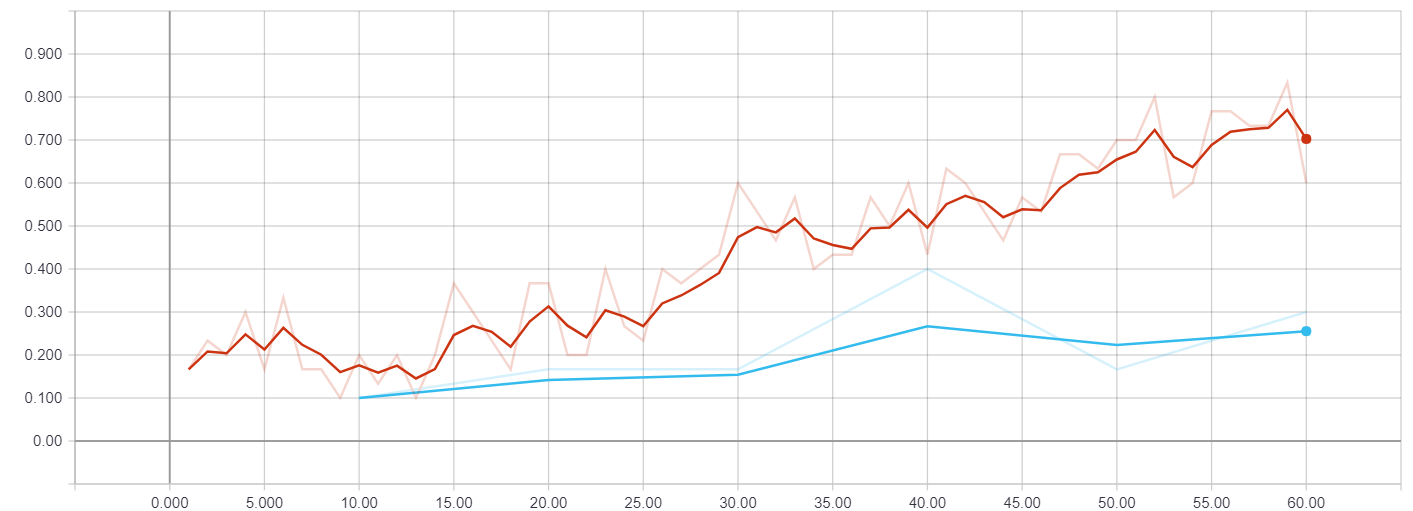
\includegraphics{imgs/augmented_model_training_acc.png}
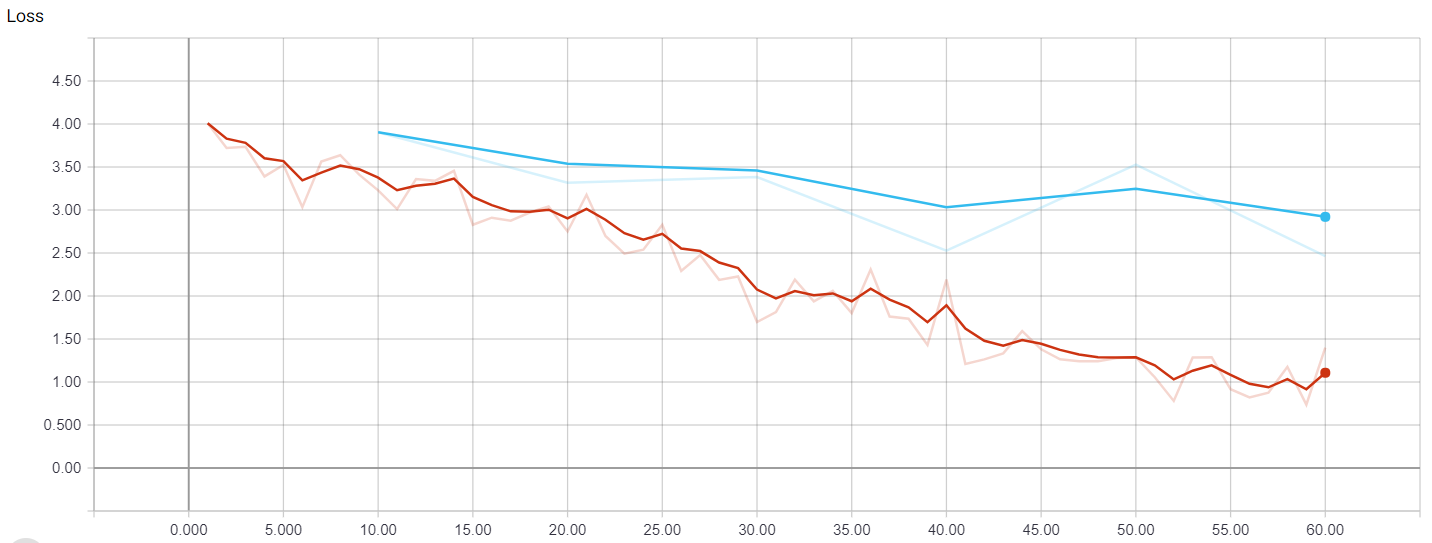
\includegraphics{imgs/augmented_model_training_loss.png}

    This is the best performing model being trained on the augmented data.

Due to the few training epochs, it is not possible to derive a
conclusion on how well the model is performing.

    \hypertarget{best-performing-model}{%
\subsubsection{Best Performing Model}\label{best-performing-model}}

    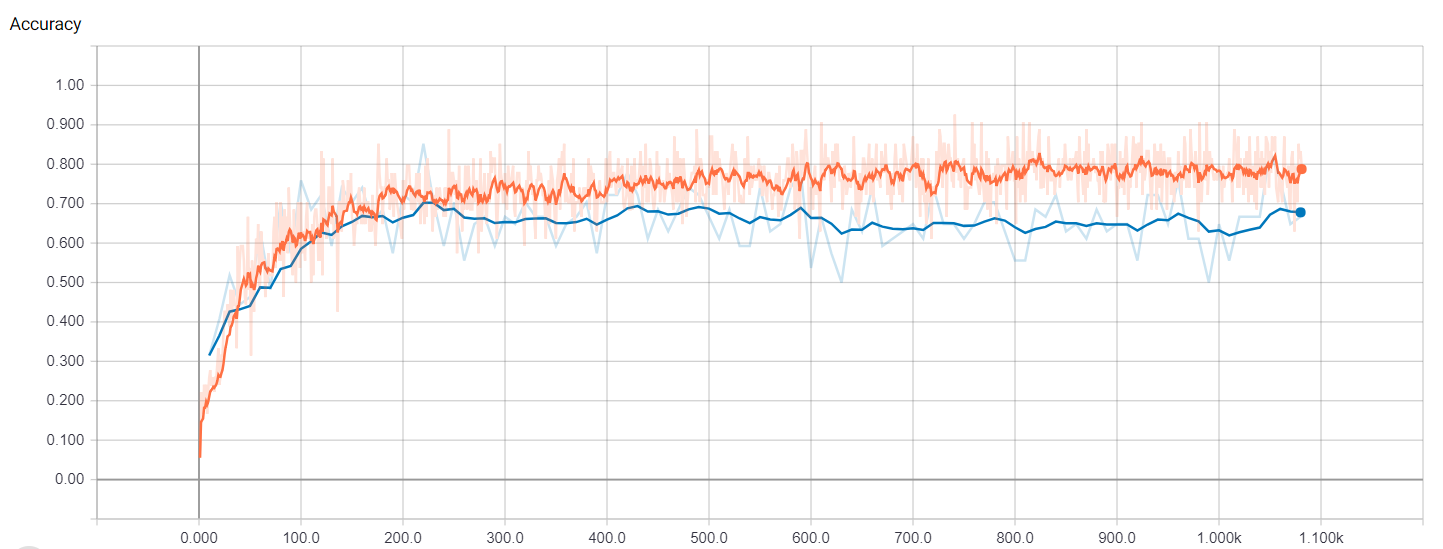
\includegraphics{imgs/best_full_model_training_acc.png}
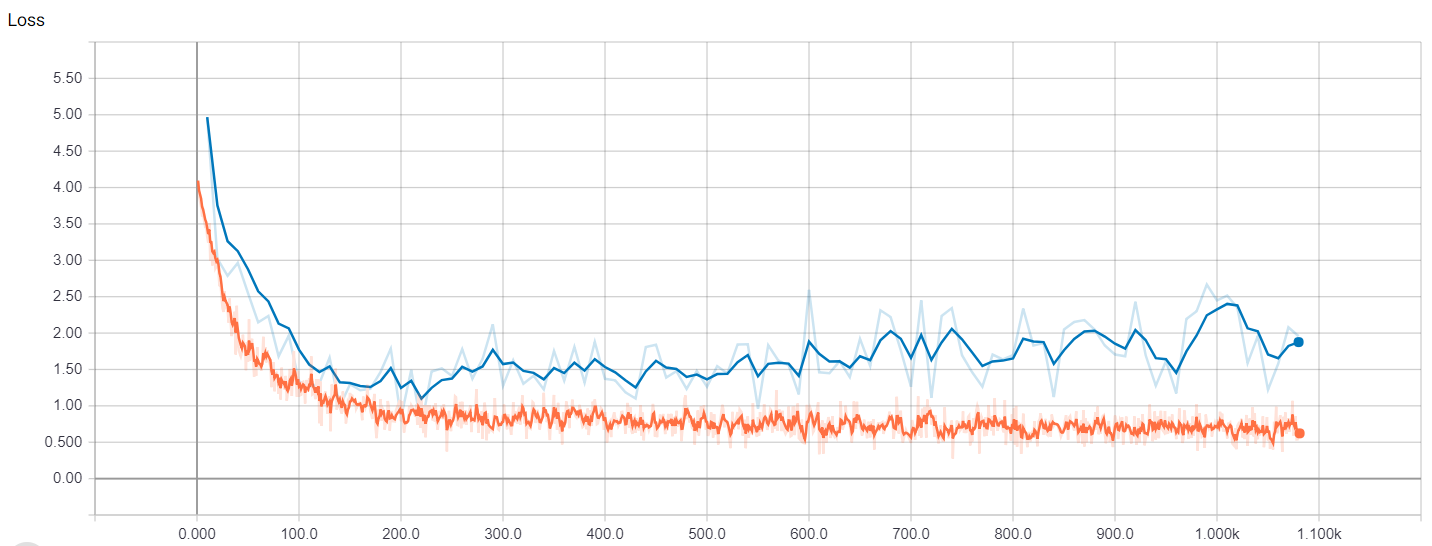
\includegraphics{imgs/best_full_model_training_loss.png}

    This is my best training.

The blue line is the validation, and the orange line is the training.
The ending accuracies are 0.7 and 0.8 for validation and training
respectively. Looking at the loss, we can see that after 1000 epochs,
the validation loss is rising, leading me to belive that the model was
overfitting. After testing the model, it was evedent that the model was
severly overfitted, having such a high difference between accuracies and
increasing validation loss.

    \hypertarget{worst-performing-model}{%
\subsubsection{Worst Performing Model}\label{worst-performing-model}}

    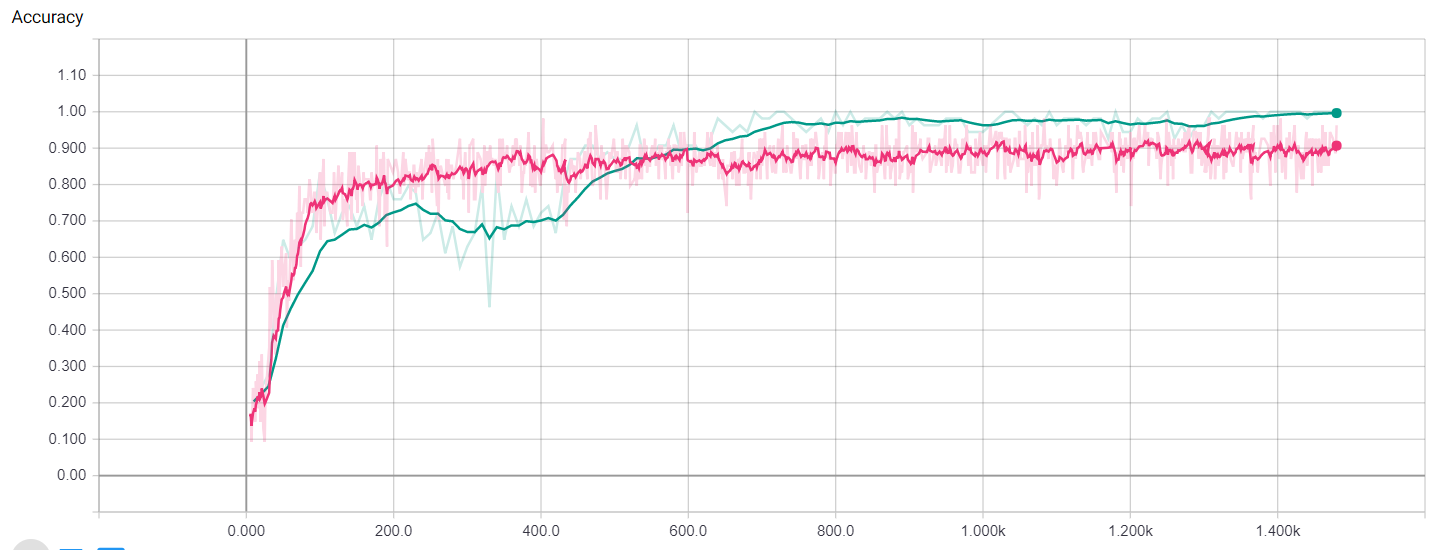
\includegraphics{imgs/underfit_full_model_training_acc.png}
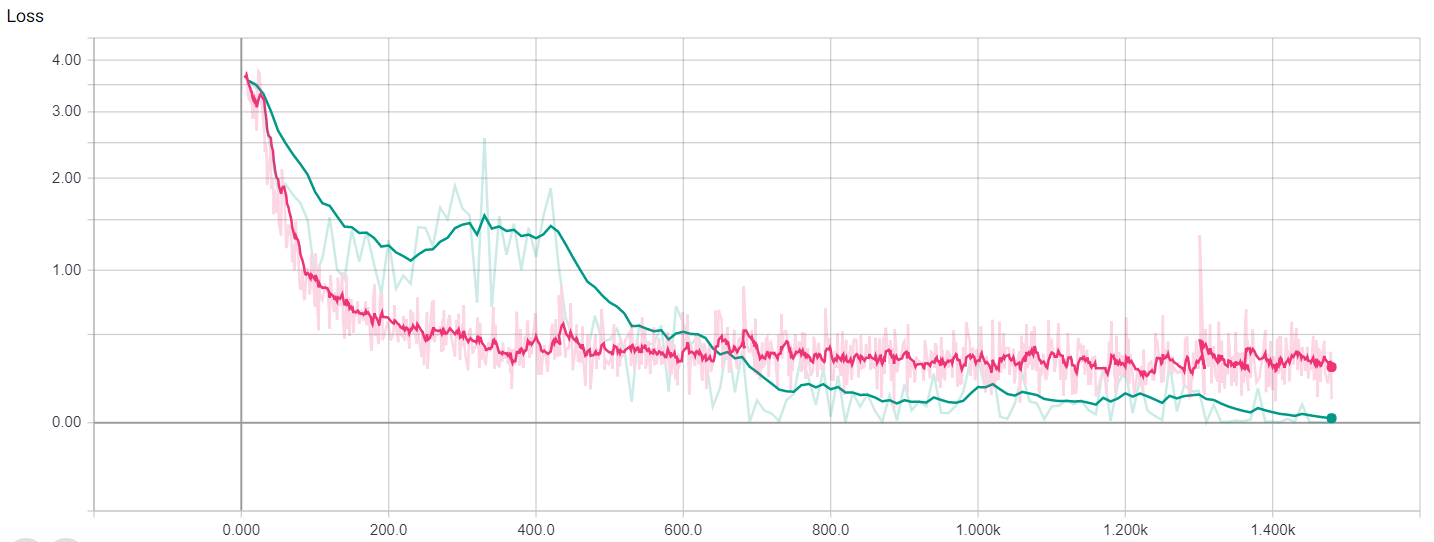
\includegraphics{imgs/underfit_full_model_training_loss.png}

    This is my worst training.

The green line is the validation, and the pink line is the training.
With the validation accuracy being higher than the training accuracy and
the valdiation loss being lower than the training loss, it is clear the
the model is underfitting. After testing the model, it was clear the the
model was unable to learn from the features.


    % Add a bibliography block to the postdoc
    
    
    
    \end{document}
